\section{Sentiment Analysis}
\label{chap:sent}
\subsection{Task definition}
\begin{itemize}
\item POS tagging \\
\textit{input}: a word \\
\textit{output}: part-of-speech tags -- as noun, pronoun, punctuation mark etc.
\item lemmatization \\
\textit{input:} a word \\
\textit{output:} lemma -- a base form of a given words, meaning for example nominative of singular for nouns or infinitive for verbs. 
\item sentiment analysis \\
\textit{input:} a sentence or a sequence of sentences \\
\textit{output:} prevailing sentiment of the input from categories: neutral, positive, negative.
\todo{doplnit diskuzi o ruzných možnostech definice}
\end{itemize}.
As stated in \citep{Veselovska}: "Sentiment analysis, also known as opinion mining, is an automatic detection of a positive or negative polarity, or neutrality of ... a text sequence", which is exactly as the sentiment analysis is understood in this work, although there are some other definitions consisting of e.g. opinion extraction, irony or stance \citep{Montoyo2012}. Another tasks related to sentiment analysis is a subjectivity analysis (whether the presented opinion is objective or highly subjective), which is also not included in this work, mainly because the lack of labelled data for Czech. It is possible to analyze individual expressions, sentences or whole documents \citep{Veselovska} and this work focuses on the document level classification.
%TODO zjistit jaka jsou na to porovnavaci data This work primary tries to improve existing tasks and show the ability of contextualized embeddings to improve results, so tasks with existing data and results were selected.  %TODO why?
\subsection{Dataset and Preprocessing}
Four main Czech datasets with sentiment annotation are available - user reviews from MALL.cz, film reviews from csfd.cz, news from Aktualne.cz and posts from czech branch pages on facebook. As Aktualnecz dataset turned out to be problematical as the text were ambiguous for annotators, and its authors later used other mentioned datasets \citep{Veselovska}, this work also focuses only on the three other data sources -- MALL, CSFD and Facebook \footnote{All three datasets are all available here: http://liks.fav.zcu.cz/sentiment/}. Following part summarize each of used datasets.
\subsubsection{Facebook}
Length: 9752\\
From: ? \\
Labels: neutral, positive, negative

\subsubsection{csfd}
Length: 91304 \\
From: \\
Labels: negative, positive ? \\

\subsubsection{mallcz}
Length: 145306 \\
From: \\
Domain: domestic appliance reviews \\
Labels: negative, neutral, positive

\subsubsection{imdb}
Length: 25000 \\
From:
Labels: negative, positive

%TODO rozlozeni trid

%TODO jak vypdaji orginalne ty labely

\begin{figure}[h]
\centering
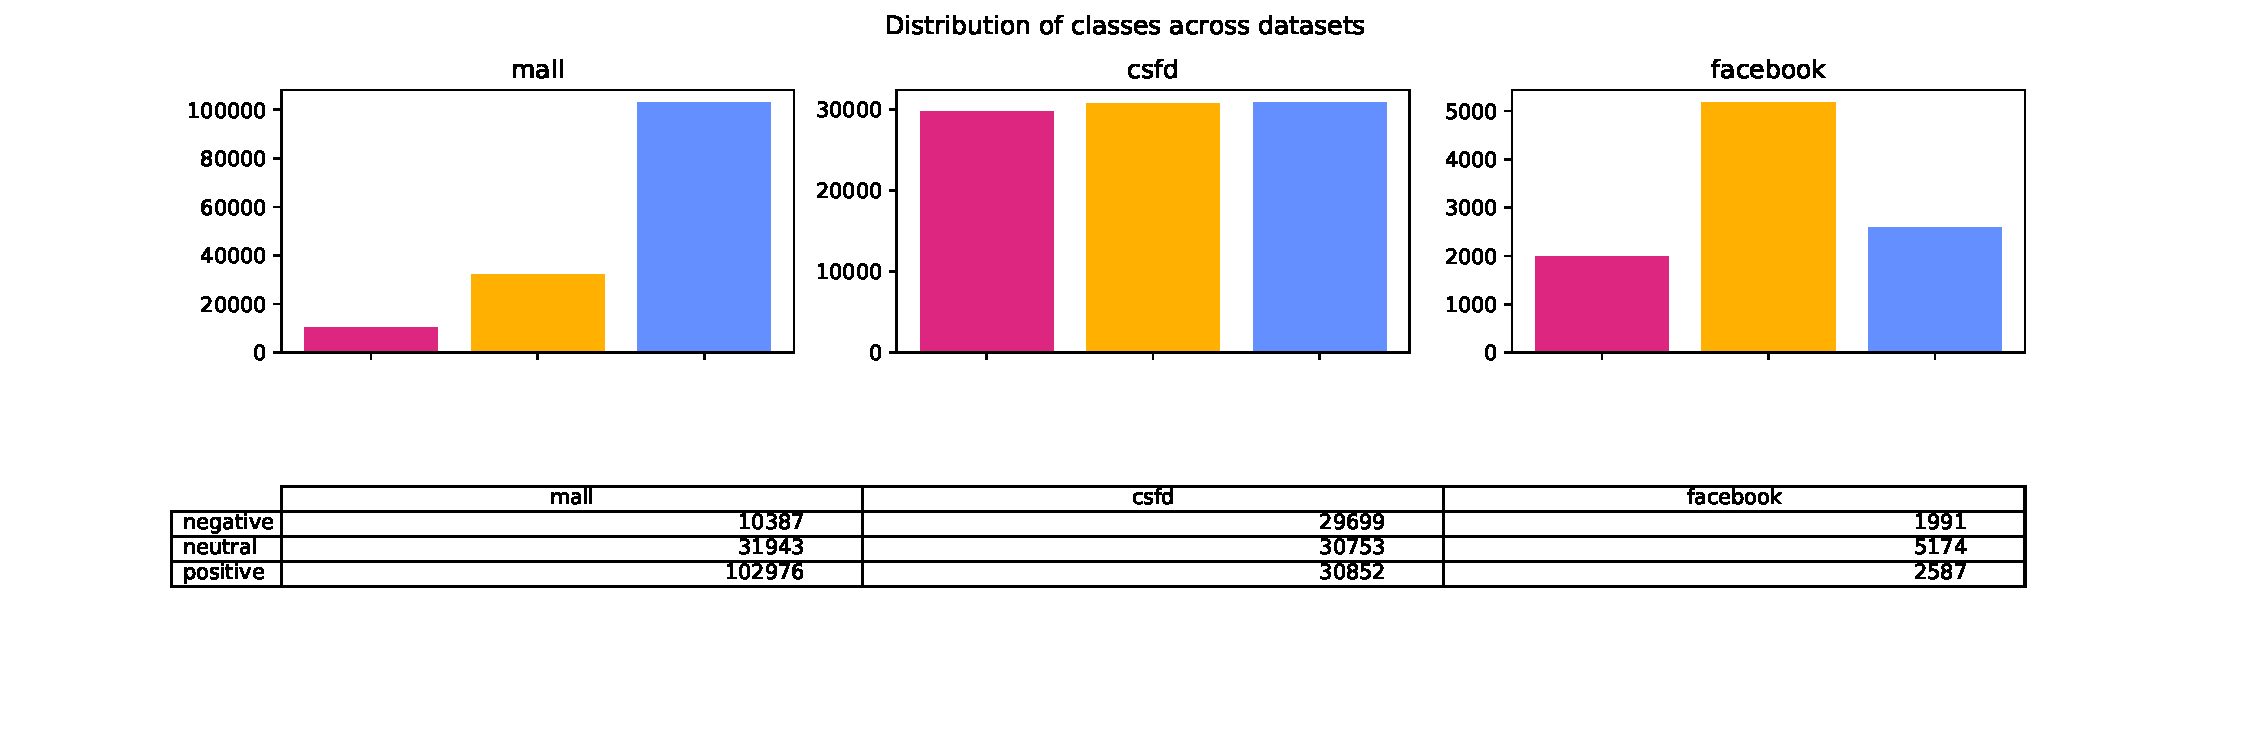
\includegraphics[width=1\columnwidth]{../img/distribution}
\protect\caption{}
\label{pic:dist}
\end{figure}

As can be seen in figure \ref{pic:dist}
distribution of labels differs among datasets. Moreover, Figure \ref{pic:dist_all}
\begin{figure}[h]
\centering
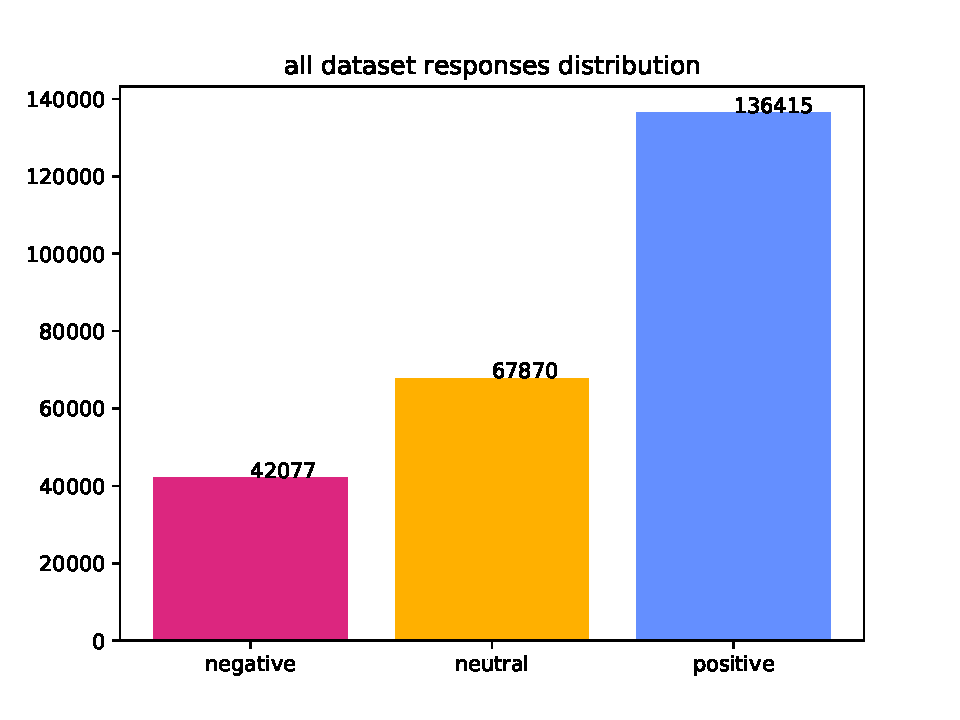
\includegraphics[width=1\columnwidth]{../img/distribution_all}
\protect\caption{}
\label{pic:dist_all}
\end{figure}
shows, that the resulting dataset is highly unbalanced, which causes divergence and stuck in training. Due to the big part of labels being positive, many learning strategies just ended with predicting only \textit{positive} class, i.e. 55\% accuracy, so unfortunately learned nothing. This was the the case for following experiments settings:
\\
learning rate of $2e-3$ for 10 epochs. This ended with predicting only one class (positive). Some progress showed the followign approach:"2:5e-5,1:2e-5, unfreezed" for facebook data only (which are balanced). This results are above 71 for accuracy (Test accuracy: 0.726
F1 metrics: 0.7077061630227595 weighted).

\subsection{Related Work}
citace:
\citep{Cano2019}
\citep{Kittask2020} .. estonian
\citep{Lenc2016} sentiment in czech
\citep{Hercig2018}
\citep{Li}
\citep{Libovicky} presents state-of-the art results in three czech NLP tasks including sentiment analysis. They use only CSFD dataset with resulting accuracy 80.8 .1 which is still not so good as Brychcín (81.5.3). The second mentioned paper, however, uses quite complicated method for classification incorporating the fact of which movie is reviewed. 

Bachelor thesis which aplies bert on sentiment analysis in czech:
%https://dspace.cvut.cz/bitstream/handle/10467/83127/F8-BP-2019-Langr-Lukas-thesis.pdf?sequence=-1&isAllowed=y
results are accuracy 84 with tfidf and about 81 with bert and they used mall dataset.




\subsection{Experiments and Architecture}
I tried another approach:
Because the facebook dataset is balanced, I pretrained the model first on facebook and after reaching a decent accuracy, i further trained the model on the join data:
for ten epochs with learning rate 5e-5 and an effecctive batch size 48.
[[ 6240 914 2783]
[ 1236 4447 529]
[ 1050 273 19020]]
Test accuracy: 0.814068837005371
F1 metrics: 0.8087903170140932

The pretraining model was obtained as:
without freezing, batch size 48, 2:5e-5,4:2e-5



Than I trained for 3 more epochs:
[[ 6599 995 2343]
[ 1246 4520 446]
[ 1470 269 18604]]
Test accuracy: 0.8145072892688808
F1 metrics: 0.8119431050948791
see \ref{pic:conf1}
\begin{figure}[h]
\centering
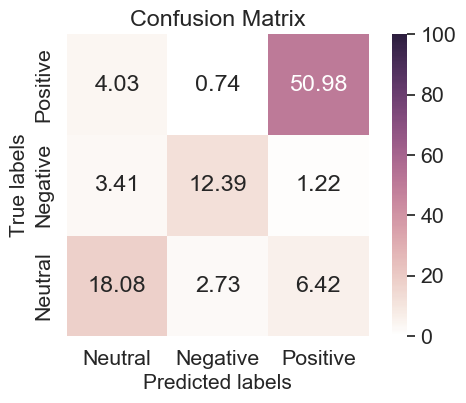
\includegraphics[width=1\columnwidth]{../img/confusion_matrix}
\protect\caption{Normalized confusion matrix}
\label{pic:conf1}
\end{figure}

\subsection{Results}

My baseline is tf-idf method, which resulted in 
[[ 4310   102  3015]
 [  685  1016   779]
 [  842    48 20227]]
              precision    recall  f1-score   support

           0       0.74      0.58      0.65      7427
           1       0.87      0.41      0.56      2480
           2       0.84      0.96      0.90     21117

    accuracy                           0.82     31024
   macro avg       0.82      0.65      0.70     31024
weighted avg       0.82      0.82      0.81     31024

0.8236526560082517 acc,


Because BERT model was trained on multilingual data, it is naturally not so good in language minoritly presented in the Bert's training data. When transfering the learned knowledge to czech sentiment task, we actually want to improve model in two ways: teach it something more specific about given task, i.e., sentiment, and improve its knowledge about selected language (czech in this case). By using czech sentiment dataset, both thing are incorporated into training. To obtained better results and following the \citep{Putra}, I also selected english sentiment dataset. The idea behind is that BERT is quite good in english and maybe can learn faster useful knowledge about the given task from data in more familiar language.














